\newpage
\section{Appendix B: Application Response}
\label{sec:Appendix B}

Appendix B constitutes the UH HASP team's official response to the feedback provided in the HASP 2019 Application review. We have addressed and answered all questions and concerns given on the application response. We have included several visuals that are up-to-date depictions of our current vision for the SORA 3 project.

For this year’s mission, we are continuing our work with the MiniPIX and astrobiology, while adding on a new project to investigate the use of hybrid-organic thin film solar cells in space. All three of our experiments are connected through the electromagnetic spectrum, with the MiniPIX and solar cell projects having a direct correlation to each other through the analysis and actual use of incident radiation, and our astrobiological unit is interested in examining the microbial life forms which survive, even thrive, in this harsh radiation environment. 

As for the astrobiology, by having a second MiniPIX mounted on the outside in free space, we are able to understand the radiation environment in which the samples that we collect exist. Part of the astrobiology mission for this year is to examine the DNA profiles of the samples collected, where we can make correlations between any mutations observed to the radiation events cataloged. 

Regarding the solar cells, we will be recording current density versus voltage graphs for the entirety of the flight, where any observed anomalies will be cross-referenced with the recorded MiniPIX data to determine the effect that cosmic rays and high energy particles have on our cells. After the flight, using electron microscopy, we will evaluate any defects caused by said high energy particles. As well we will be observing the spectrum of light incident on our payload using photodiodes. 

As to why we to added the organic solar cell unit into the mix; we want to continue doing research in semiconductor physics related to space. With nanophysics growing exponentially, organic semiconducting devices are a hot topic. We believe that organic and hybrid organic photovoltaic (HOPV) devices will play a critical role in the future of space energy harvesting, and the HASP platform provides a perfect environment to analyze these cells in situ. 

Finally, we are adding a second MiniPIX onto our payload to be housed in a box replicating the radiation shielding used on the International Space Station in order to determine the radiation environment to which astronauts are exposed. By having both MiniPIX devices we can then determine exactly what kind of radiation was effectively shielded.


\subsection{Payload Design}

We have made slight modifications to our power and weight budget, as well as added the uncertainty in the values. These changes are reflected in Table \ref{tab:PWBudget-Updated}. The total current consumption listed on this table is an estimation for the maximum current draw possible from our payload. As it can be seen, our estimated current and weight consumption falls well within the specified limits established by HASP.

Figure \ref{fig:PayloadDrawing-Updated} addresses the height violation presented in our original application.
The extension of the astrobiology T-arm has been reduced so that the lid remains within the height limit of \SI{300}{\milli\meter}.
As a result, we will not be requesting a height wavier.

Our payload footprint overlayed on the HASP mounting plate is explicitly shown in the Figure \ref{fig:PayloadFootprint} along with the closest distances between the SORA 3 payload and the boundaries set by HASP.
Also shown in Figure \ref{fig:PayloadFootprint} is the requested direction of orientation of our payload.
We do not have a preference to where our payload is placed on the central structure.

\subsection{Electronics}

The baud rate for all serial communication will be set to 4800 bits per second. To utilize serial commands, the DB9 connection will feed into an RS232 to TTL converter which will then be read by our flight computer.

The electronics diagram presented in Figure \ref{fig:WiringDiagram-Updated}  has been updated to provide a more detailed and accurate depiction of our current system plans.
The updated diagram features the voltage required by each device for operation and the data lines from each device.

As suggesting by a reviewer, will utilize the serial commands shown in Table \ref{tab:SerialCommands}. These commands will serve as backup to the discrete commands presented in the original application.

\subsection{Team Structure}

Additionally, the team structure had a slight modification.
We had a change in position of electronics coordinator, and Figure \ref{fig:TeamRoleTree-Updated} reflects the change in this leadership role.

\newpage

\begin{table}[H]
  \centering
  \caption{Updated power and weight budget for SORA 3.} 
  \label{tab:PWBudget-Updated}
  \bigskip
  \begin{tabular}{cccccc}
    \hline
    \hline
    \multicolumn{1}{c}{\bfseries Component} & \multicolumn{1}{c}{\bfseries Voltage (\si{\volt}DC)} &  \multicolumn{1}{c}{\bfseries Current (\si{\milli\ampere})} & \multicolumn{1}{c}{\bfseries Duty Cycle (\%)} & \multicolumn{1}{c}{\bfseries Power (\si{\milli\watt})} & \multicolumn{1}{c}{\bfseries Mass (\si{\gram})} \\
    \hline
    30-5 \si{\volt} DC/DC Supply & 30 & N/A & 100 & N/A & 68 $\pm$ 2 \\
    RP3 + (2)MiniPIX & 5 & 1210 $\pm$ 100 & 100 & 6050 $\pm$ 500 & 92.4 $\pm$ 5 \\    
    Linear Actuator & 12 & 185 $\pm$ 20 & 20 & 2220 $\pm$ 240 & 40 $\pm$ 5 \\
    Stepper Motor & 6.2 & 800 $\pm$ 50 & 100 & 4960 $\pm$ 310 & 50 $\pm$ 5 \\
    Accelerometer & 5 & 3.9 $\pm$ 1 & 100 & 19.5 $\pm$ 5 & 10 $\pm$ 2 \\
    (3)Photodiodes & 3.6 & 1.8 $\pm$ 0.5 & 100 & 6.48 $\pm$ 1.8 & 15 $\pm$ 5 \\
    (14)Thermistors & 5 & 3.5 $\pm$ 0.5 & 100 & 17.5 $\pm$ 2.5 & 70 $\pm$ 5 \\
    Pressure Sensor & 3.6 & 1.4 $\pm$ 0.5 & 100 & 5.04 $\pm$ 1.8 & 2 $\pm$ 0.1 \\
    Low Pressure Sensor & 5 & 7 $\pm$ 1 & 100 & 35 $\pm$ 5 & 2 $\pm$ 0.1 \\   
    \SI{12}{\volt} Step-up & 2.5 - 12 & N/A & 100 & N/A & 0.4 $\pm$ 0.1 \\

    Structure w/ bolts & N/A & N/A & N/A & N/A & 5000 \\
    \hline
    \textbf{Total} & N/A & \textbf{2212.6 $\pm$ 173.5} & N/A & \textbf{13313.52 $\pm$ 1066.1} & \textbf{5349.8 $\pm$ 529.3}  \\
    \hline
    \hline
  \end{tabular}
  \medskip
\end{table}

\begin{figure}[H]
  \centering
  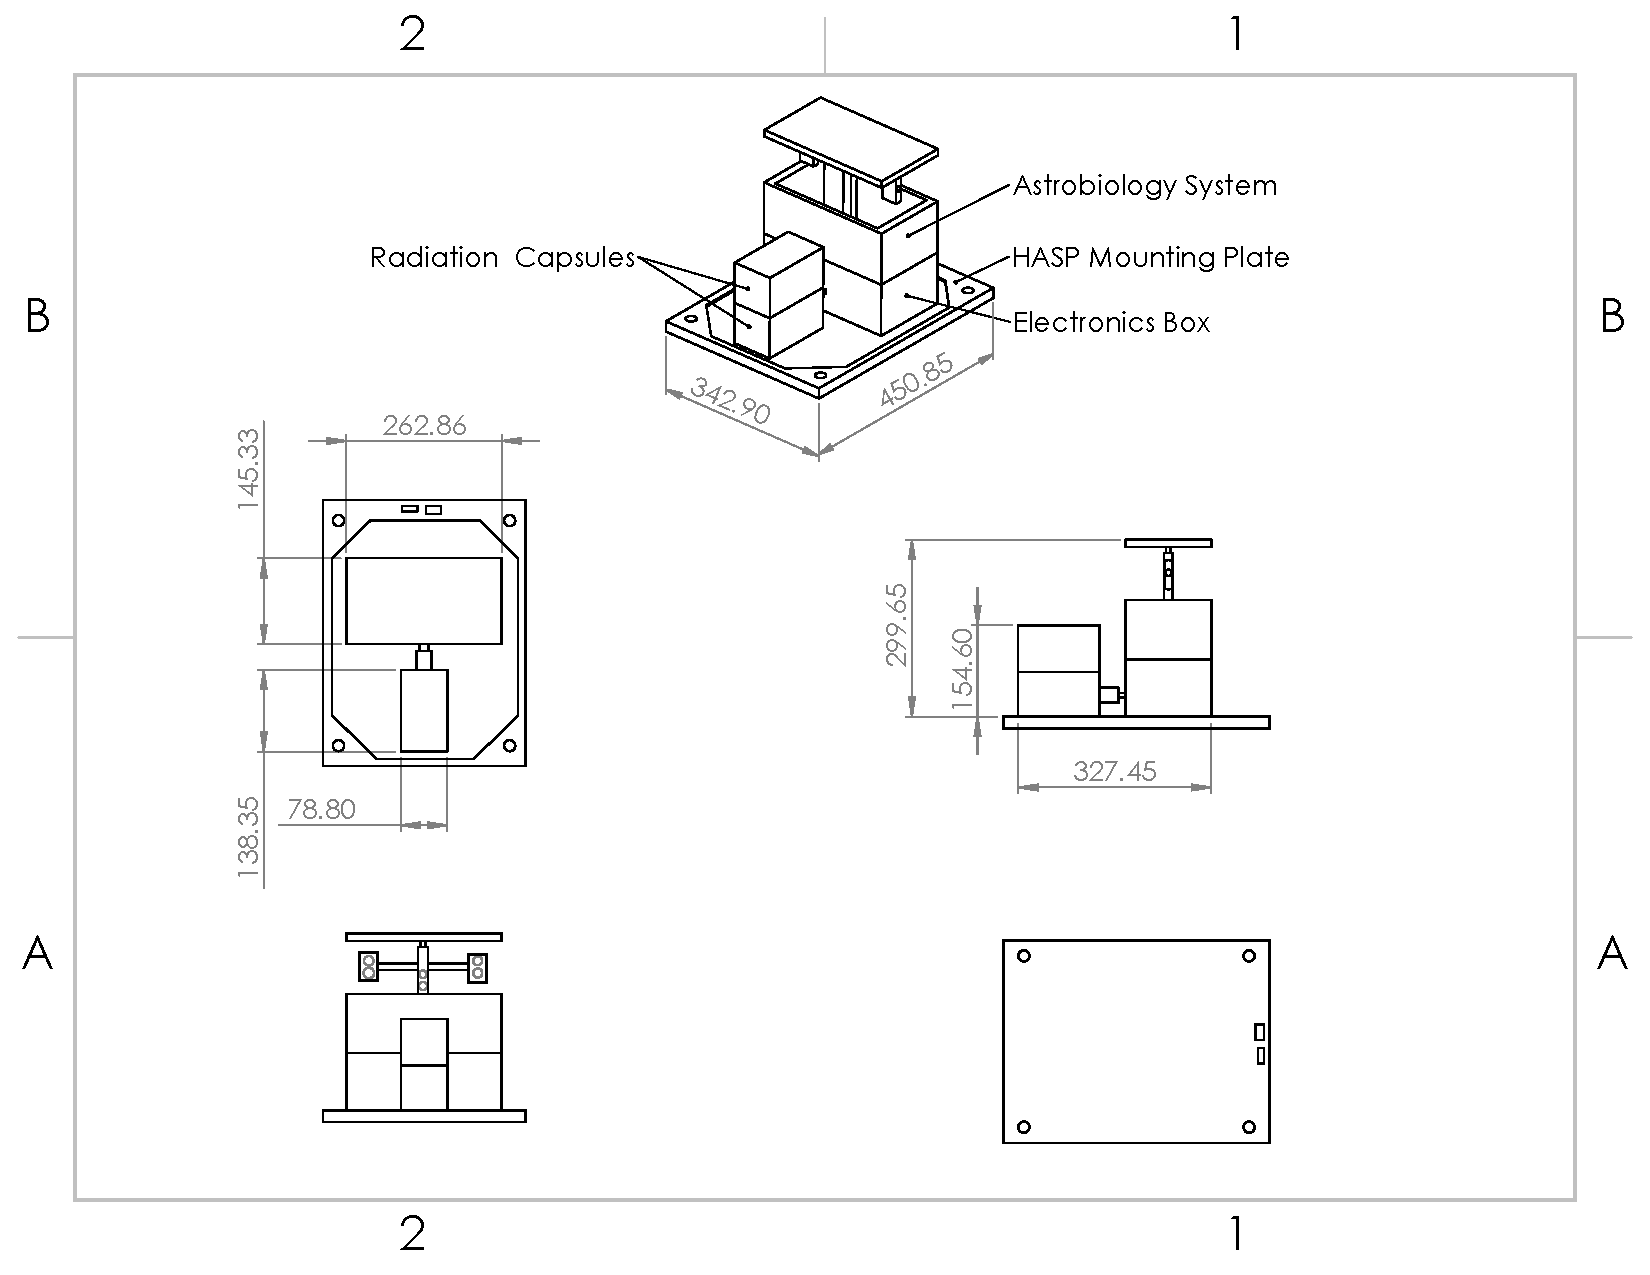
\includegraphics[width=\textwidth]{./Figures/PayloadDrawing-Updated.pdf}
  \caption{Updated drawing for the preliminary payload design featuring new dimensions, positioning, and labels. All dimensions are in millimeters.}
  \label{fig:PayloadDrawing-Updated} 
\end{figure}

\begin{figure}[H]
  \centering
  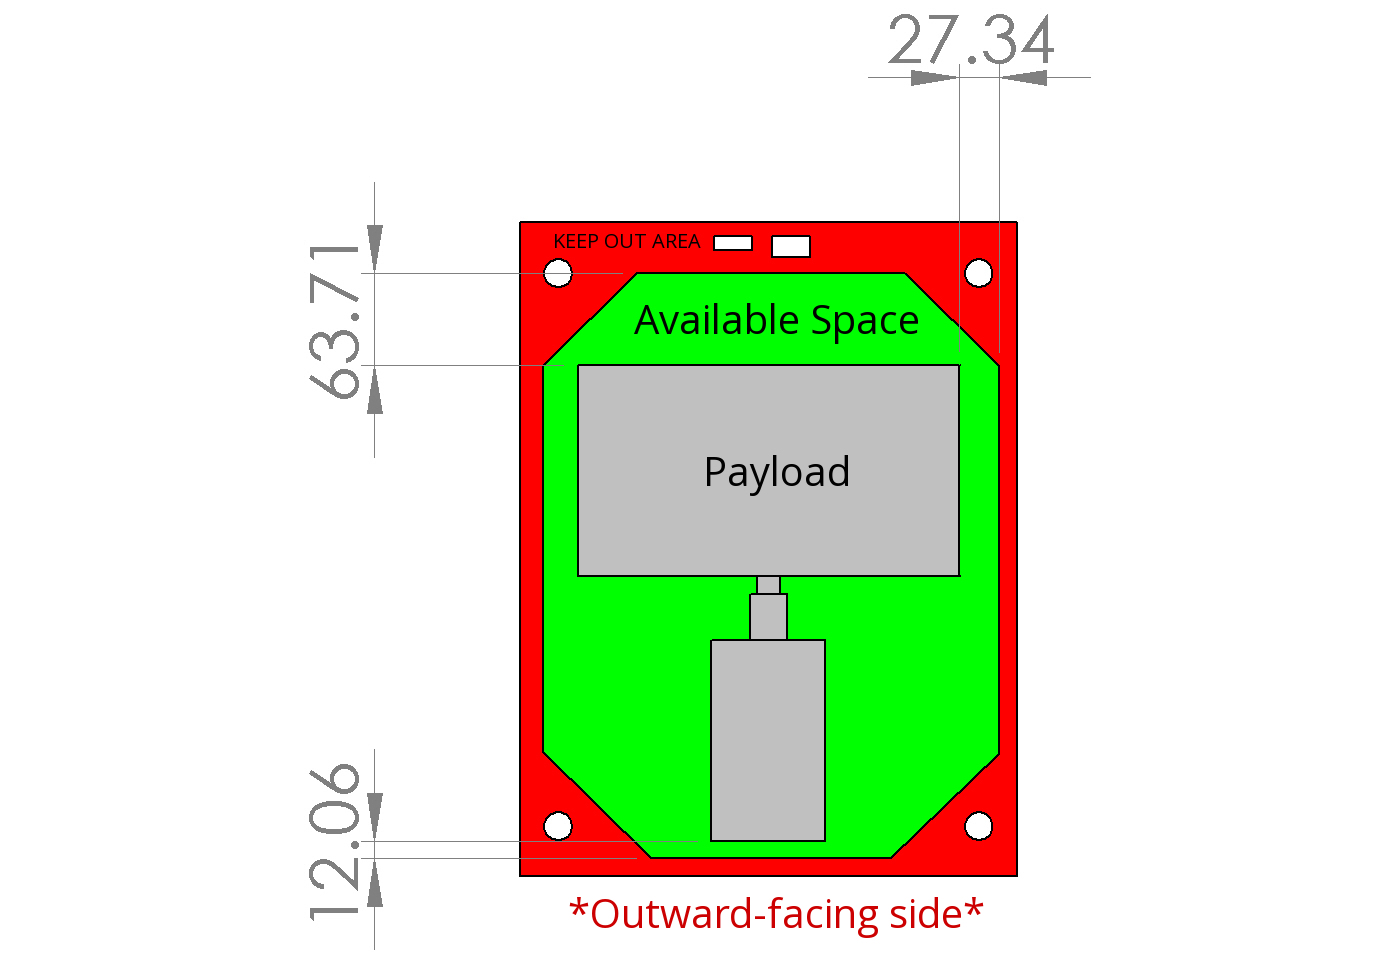
\includegraphics[width=\textwidth]{./Figures/PayloadFootprint.jpg}
  \caption{Depiction of the payload's footprint on the HASP mounting plate. All dimensions are in millimeters.}
  \label{fig:PayloadFootprint} 
\end{figure}

\begin{figure}[H]
  \centering
  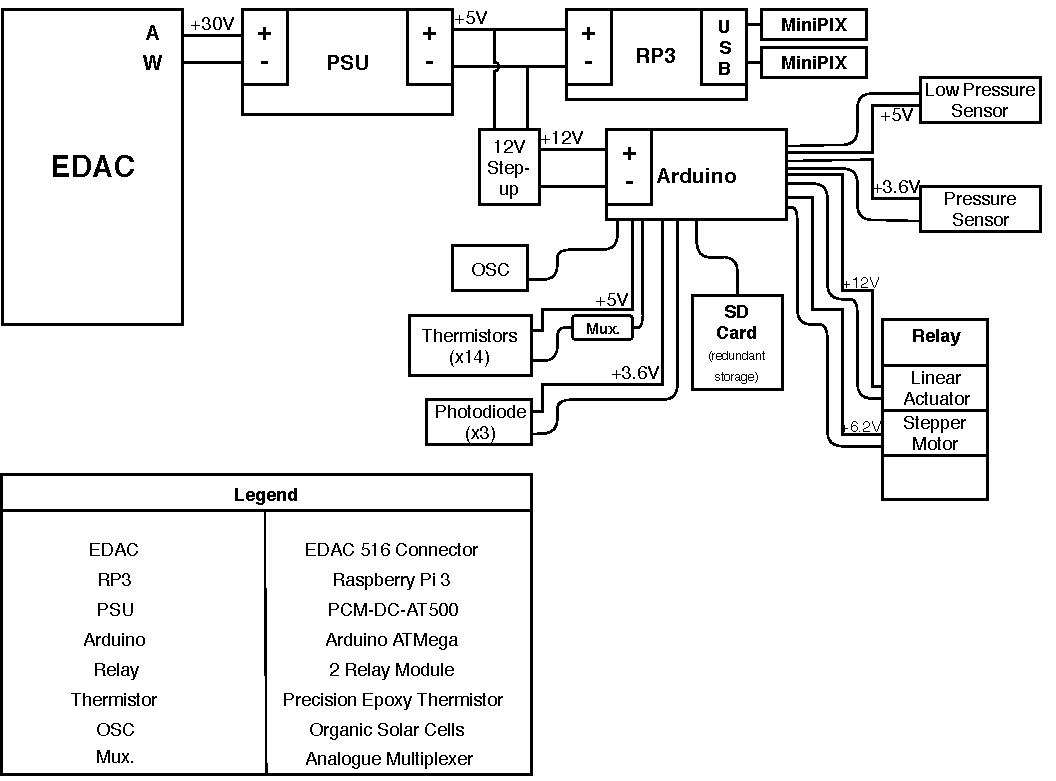
\includegraphics[width=\textwidth]{./Figures/WiringDiagram-Updated.pdf}
  \caption{Updated wiring diagram for the SORA 3 payloaf. Power lines are depicted as the sharp-edged lines, and the data lines are depicted as the curved lines.}
  \label{fig:WiringDiagram-Updated} 
\end{figure}

\begin{table}[H]
  \centering
  \caption{Updated power and weight budget for SORA 3.} 
  \label{tab:SerialCommands}
  \bigskip
  \begin{tabular}{cc}
    \hline
    \hline
    \multicolumn{1}{c}{Command} & \multicolumn{1}{c}{HEX Command} \\
    \hline
    Start astrobiology system & 0x01 \\
    Stop astrobiology system & 0x02 \\
    Start electronics system & 0x03 \\
    Stop electronics system & 0x04 \\
    \hline
    \hline
  \end{tabular}
\end{table}

\begin{figure}[H]
  \centering
  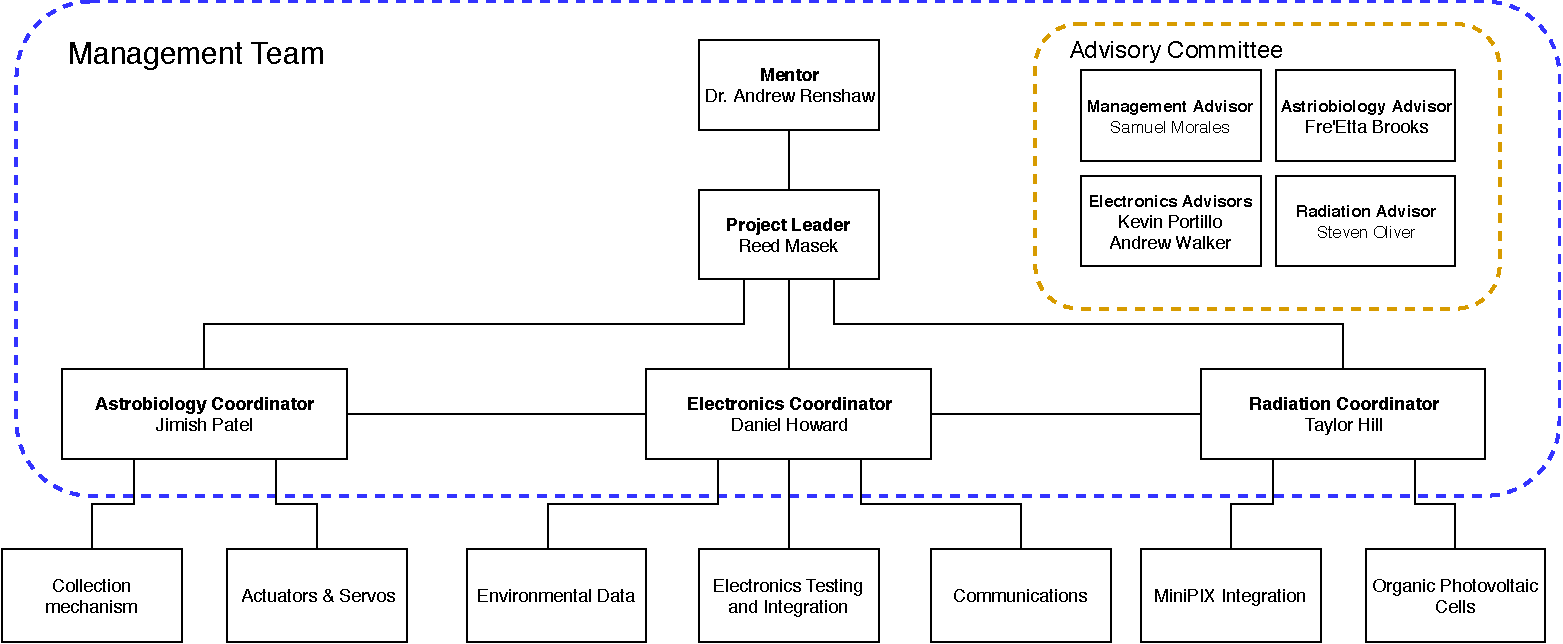
\includegraphics[width=\textwidth]{./Figures/TeamRoleTree-Updated.pdf}
  \caption{Updated team tree reflecting the change in electronics coordinator.}
  \label{fig:TeamRoleTree-Updated} 
\end{figure}

\newpage